 \documentclass[12pt,letterpaper]{article}
\usepackage[utf8]{inputenc}
\usepackage[spanish, es-tabla]{babel}
\usepackage[version=3]{mhchem}
\usepackage[journal=jacs]{chemstyle}
\usepackage{amsmath}
\usepackage{amsfonts}
\usepackage{amssymb}
\usepackage{makeidx}
\usepackage{xcolor}
\usepackage{verbatim}
\usepackage[stable]{footmisc}
\usepackage[section]{placeins}
%Paquetes necesarios para tablas
\usepackage{longtable}
\usepackage{array}
\usepackage{xtab}
\usepackage{multirow}
\usepackage{colortab}
%Paquete para el manejo de las unidades
\usepackage{siunitx}
\sisetup{mode=text, output-decimal-marker = {,}, per-mode = symbol, qualifier-mode = phrase, qualifier-phrase = { de }, list-units = brackets, range-units = brackets, range-phrase = --}
\DeclareSIUnit[number-unit-product = \;] \atmosphere{atm}
\DeclareSIUnit[number-unit-product = \;] \pound{lb}
\DeclareSIUnit[number-unit-product = \;] \inch{"}
\DeclareSIUnit[number-unit-product = \;] \foot{ft}
\DeclareSIUnit[number-unit-product = \;] \yard{yd}
\DeclareSIUnit[number-unit-product = \;] \mile{mi}
\DeclareSIUnit[number-unit-product = \;] \pint{pt}
\DeclareSIUnit[number-unit-product = \;] \quart{qt}
\DeclareSIUnit[number-unit-product = \;] \flounce{fl-oz}
\DeclareSIUnit[number-unit-product = \;] \ounce{oz}
\DeclareSIUnit[number-unit-product = \;] \degreeFahrenheit{\SIUnitSymbolDegree F}
\DeclareSIUnit[number-unit-product = \;] \degreeRankine{\SIUnitSymbolDegree R}
\DeclareSIUnit[number-unit-product = \;] \usgallon{galón}
\DeclareSIUnit[number-unit-product = \;] \uma{uma}
\DeclareSIUnit[number-unit-product = \;] \ppm{ppm}
\DeclareSIUnit[number-unit-product = \;] \eqg{eq-g}
\DeclareSIUnit[number-unit-product = \;] \normal{\eqg\per\liter\of{solución}}
\DeclareSIUnit[number-unit-product = \;] \molal{\mole\per\kilo\gram\of{solvente}}
\usepackage{cancel}
%Paquetes necesarios para imágenes, pies de página, etc.
\usepackage{graphicx}
\usepackage{lmodern}
\usepackage{fancyhdr}
\usepackage[left=4cm,right=2cm,top=3cm,bottom=3cm]{geometry}

%Instrucción para evitar la indentación
%\setlength\parindent{0pt}
%Paquete para incluir la bibliografía
\usepackage[backend=bibtex,style=chem-acs,biblabel=dot]{biblatex}
\addbibresource{references.bib}

%Formato del título de las secciones

\usepackage{titlesec}
\usepackage{enumitem}
\titleformat*{\section}{\bfseries\large}
\titleformat*{\subsection}{\bfseries\normalsize}

%Creación del ambiente anexos
\usepackage{float}
\floatstyle{plaintop}
\newfloat{anexo}{thp}{anx}
\floatname{anexo}{Anexo}
\restylefloat{anexo}
\restylefloat{figure}

%Modificación del formato de los captions
\usepackage[margin=10pt,labelfont=bf]{caption}

%Paquete para incluir comentarios
\usepackage{todonotes}

%Paquete para incluir hipervínculos
\usepackage[colorlinks=true, 
            linkcolor = blue,
            urlcolor  = blue,
            citecolor = black,
            anchorcolor = blue]{hyperref}

%%%%%%%%%%%%%%%%%%%%%%
%Inicio del documento%
%%%%%%%%%%%%%%%%%%%%%%

\begin{document}
\title{Instituto Tecnológico de Costa Rica\\Control Automático EL-5408\\Proyecto Introductorio}
\author{Alexander Alvarado Sotela\\2016180346\\Esteban González Fernández \\201112358\\José Pablo Quesada Quesada\\2014115933\\Julio C. Viveros Hernandez\\200946192}
\date{5 de septiembre, 2019}
\maketitle
\section{Objetivos}
\begin{enumerate}
\item Encontrar la ecuación de transferencia a partir de la ecación que modela el sistema.
\item Encontrar el error del sistema para lazo abierto y lazo cerrado. 
\item Determinar el lugar de las raíces para el sistema. 
\item Encontrar reguladores que permitan obtner condiciones de sobreimpulso y amortiguamiento deseadas.
\item Diseñar reguladores de atraso y adelanto para cumplir con condiciones de error y tiempo de estabilización deseades. 
\item Utilizar la herramienta Máxima para representar el lugar de las raíces y las respuestas del sistema con los distintos compensadores.
\end{enumerate} 
 
 
\section{Descripción del Sistema a Analizar} 
Los sistemas de control automático se utilizan en distintas aplicaciones, su gran importancia es la capacidad de brindar realimentación de las señales a controlar y poder regularlas para obtener las salidas deseadas.  
Uno de las métodos para lograr esta regulación es utilizar el lugar de las raíces, este método consiste en encontrar las raíces de la ecuación característica del sistema y ubicar los polos y ceros en los lugares deseados haciendo uso de un regulador y en caso de ser necesario compensadores. 
Los compensadores pueden ser de atraso o adelanto dependiendo de las variables que se deseen controlar, si se requiere variar el error se coloca un compensador de atraso, si se requiere variar el tiempo de estabilziación se coloca un compensador de adelanto.
 El sistema a analizar corresponde a un torno paralelo convencional, el cual está descrito por cuatro elementos
\begin{enumerate}
    \item Motor de corriente directa: \\ 
    \begin{equation}
    G_{1}(s) = \frac{1}{s^{2}+8s+6}
    \end{equation}
    \item  Sistema de engranes de transmisión:\\ 
    \begin{equation}
    G_{2}(s) = \frac{1}{2}
    \end{equation}
    \item  Acoplamiento: 
    \begin{equation}
    G_{3}(s) = \frac{1}{s}
    \end{equation}
    \item Modelo del carro longitudinal: \\
    \begin{equation}
    G_{4}(s) = \frac{1}{s^{2}+8s+25}
    \end{equation}
\end{enumerate}
 El sistema debe contar con un regulador que permita obtener un comportamiento similar a un sistema de segundo orden subamortiguado con un sobreimpluso del 5\% ante una entrada escalón unitario. Luego se debe adicionar al sistema un compensador de atraso para reducir el error de estado estacionario al menor valor posible. 
 Por último se debe sustituir el compensador de atraso por un compensador de adelanto para obtener un tiempo de estabilización menor a 0,1s. 


 \begin{figure}[H]
            \centering
            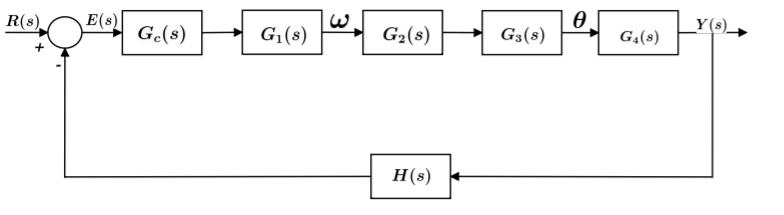
\includegraphics{DiagramaBloques.PNG}
            \caption{ Diagrama de bloques del sistema.}
            \label{files}
\end{figure} 

\section{Obtención del modelo matemático}

 Inicialmente se procede a obtener la función de transferencia del sistema en lazo abierto, donde se obtiene lo siguiente:\\

\begin{equation}
    \frac{1}{2s(2s+8s+6)(2s+8s+25)(s+3)}
    \label{tla}
\end{equation}

Se procede a obtener la función de transferencia del sistema a lazo cerrado. Se conoce que la función de transferencia a lazo cerrado debe ser:

\begin{equation}
    \frac{G_{T}(s)}{1+G_{T}(s)H(s)}
    \label{form}
\end{equation}
Donde en la ecuación \ref{form} $G_{T}(s)$ es la multiplicación de todos los diagramas de bloque.
Por lo que tenemos la siguiente deducción matemática:

$$\frac{\displaystyle \frac{K_{c}}{2s(s+3)(s+2)(s+4+3j)(s+4-3j)}}{\displaystyle 1+\frac{K_{c}}{2s(s+3)^{2}(s+2)(s+4+3j)(s+4-3j)}} $$\\

Donde si simplificamos matemáticamente, logramos obtener la siguiente función de transferencia en lazo cerrado:

\begin{equation}
    \frac{K_{c}(s+3)}{2s(s+3)(s+2)(s+4+3j)(s+4-3j)+K_{c}}
    \label{tlc}
\end{equation}\\

Ahora, contando con las ecuaciones \ref{tla} y \ref{tlc} se procede a calcular el error del sistema
\begin{equation}
    {E_{o}=(1 - G(s))R(s)}
    \label{Error}
\end{equation}
Seguidamente, en la ecuación \ref{Error} sustituimos los valores de G(s) y R(s) por los datos que tenemos de función de transferencia y entrada un escalón unitario en el dominio de laplace
$${E_{o}=(1 - \frac{K_{c}}{2s(s+3)(s+2)(s+4+3j)(s+4-3j)+K_{c}})\frac{1}{s}}$$

\begin{equation}
    {E_{o}=(\frac{1}{s} - \frac{K_{c}}{2s^{2}(s+3)(s+2)(s+4+3j)(s+4-3j)+K_{c}})}
    \label{Error1}
\end{equation}

Dentro de los requerimientos se solicita calcular el regulador que permita permita obtener un comportamiento similar a un sistema de segundo orden subamortiguado con un sobreimpluso del 5\% ante una entrada escalón unitario. El proceso seguido para el cálculo se muestra a continuación.

Para el diseño de un compensador de adelanto, se debe tener muy en cuenta los requisitos de diseño, en este caso ya mencionados, para posteriormente, determinar con dichos valores los polos dominantes del sistema de segundo orden deseado cuyo comportamiento queremos caracterizar en la planta.

Necesitamos que el sistema sea amortiguado, por lo cual, sabemos que el $\zeta$ debe estar entre 0 y 1. Ahora, también necesitamos que el sobreimpulso no exceda en un 5\%, por lo que podemos calcular el valor de $\zeta$ mediante la siguiente ecuación

\begin{equation}
    {\zeta = \sqrt{\frac{\ln{(\frac{5}{100})^{2}}}{\ln{(\frac{5}{100})^{2}+\pi^{2}}}}=0,69 \approx 0,7}
    \label{Chi}
\end{equation}

De la ecuación \ref{Chi} obtenemos que el valor para $\zeta$ es de 0.69, sin embargo, utilizaremos la aproximación del valor a 0,7 para trabajar con valores exactos. Posteriormente seleccionamos un valor de $\omega_{n}$ (frecuencia natural no amortiguada) de 4rad/s, lo cual con este dato junto con el valor $\zeta$ encontrado en \ref{Chi}, podemos calcular los datos como tiempo de estabilización y los polos dominantes del sistema de segundo orden subamortiguado que queremos encontrar.

\begin{equation}
    {t_{s}=\frac{4}{\zeta\omega_{n}}=1,4285seg}
    \label{ts}
\end{equation}
La forma que debe tener la ecuación que genera los polos dominantes está dada por
\begin{equation}
    {s^{2}+2\zeta\omega_{n}s+\omega_{n}^{2}}
    \label{poldom}
\end{equation}
Y de \ref{poldom} obtenemos las raíces que producen los polos domintantes
\begin{equation}
    {\widehat{r}_{1,2}} = {-2,8\pm j\frac{2\sqrt{51}}{5}}
    \label{rootsD}
\end{equation}
Como se quiere diseñar un compensador de adelanto, dado los polos dominantes obtenidos en \ref{rootsD}, se procede a proponer primero un cero estratégico y posteriormente, a partir de ese cero propuesto, encontrar la ubicación del polo del compensador.

El cero que se escoge es en $s=-2$ debido a que de esa manera, podemos cancelar ese cero con el polo ubicado en ese mismo punto. Por otra parte, una vez definido la ubicación de este cero, se utiliza la condición de fase para determinar el ángulo que debe tener el polo del compensador con respecto al polo dominante para poder encontrar su ubicación. Dicha condición de fase está dada por 
\begin{equation}
    {\phi_{z}-\theta_{z}+\phi_{p}-\theta_{p}=\pm 180^{o}(2k+1); k=0,1,2... }
    \label{condAngulos}
\end{equation}
Donde los ángulos con indice z corresponden a los del compensador y los ángulos con índice p corresponden a los de la planta, además, los ángulos $\phi$ corresponden a los ceros y $\theta$ al de los polos.

Es importante saber que, si se está diseñando un compensador de adelanto, el ángulo del cero con respecto a la horizontal en sentido contrario al giro del reloj, debe ser mayor al ángulo del polo, lo que quiere decir que el polo va a estar más alejado del origen con respecto al cero sobre el eje x negativo. Esto es importante tenerlo en cuenta ya que es de mucha utilidad para saber si los polos encontrados para el compensador son correctos o no.

Los resultados de los ángulos obtenidos son los siguientes
$$
\begin{array}{|@{}l|c|}
     \hline\phi_{z}  & 0 & & \\
     \theta_{z}  & x & & \\
     \phi_{p}  & 0 & & \\
     \theta_{p}  & 306.42^{o} & & \\
     \hline
\end{array}
$$
En el cuadro anterior podemos observar los valores de los ángulos obtenidos. Note que $\theta_{z}$ es el valor del ángulo del polo del compensador (el ángulo que se desea encontrar), y $\phi_{z}$ es cero, ya que a como habíamos mencionado, ese cero se escogió estratégicamente para cancelar con un polo de la función de transferencia, así, ambos ángulos no se toman en cuenta para el cálculo de los ángulos.
\begin{equation}
    {\theta_{z}=180^{o}(2k+1)-306.42^{o}=233.58^{o}}
    \label{anguloCompensador}
\end{equation}
Aplicando trigonometría, se obtiene que el valor del polo debe ser
\begin{equation}
    {s_{p}=-4,9076}
    \label{PoloCompensador}
\end{equation}
En este punto ya tenemos los valores del polo y del cero para el compensador de adelanto, por lo que podemos expresar el compensador como
\begin{equation}
    \frac{K_{c}(s+2)}{s+4,9076}
    \label{Compensador}
\end{equation}

Como resultado se obtiene un $K_{c}=3$ que cumple con los requisitos de diseño.

Para cumplir con el requerimiento de un tiempo de estabilización menor a 0,1$s$ solicitado en uno de las nuevas condiciones de diseño, se utiliza un compensador de adelanto (el compensador de atraso no se toma en cuenta para esta solución), el mismo fue calculado de la siguiente manera

$$
    {t_{s}<0,1seg}\\
$$
Para un valor de $t_{s}$ igual a 0,1seg con un coeficiente de amortiguamiento de 0,7 se obtiene el siguiente de frecuencia natural no amortiguada
$$
    \omega_{n}=\frac{4}{\zeta t_{s}}\\
$$
$$
    \omega_{n}=\frac{4}{(0,7)(0,1seg)}=\frac{400}{7}\\
$$
\begin{equation}
\\
    \omega_{n}\approx 57,14rad/seg
    \label{FrecNueva}
\end{equation}

De aquí, al realizar los mismos cálculos para determinar el polo y el cero del compensador, se llega a los siguientes valores de ubicación del cero y del polo

\begin{equation}
    z = -60
    \label{zerNuevo}
\end{equation}

\begin{equation}
    p = -84,65
    \label{polNuevo}
\end{equation}

Por lo tanto, el nuevo compensador, conservando el $K_{c}$ obtenido en el punto 5, se llega a que el compensador de adelanto diseñado es el siguiente

\begin{equation}
    G_{c2}=\frac{K_{c}(s+60)}{s+84,65}
    \label{CompNuevo}
\end{equation}

Analizando críticamente los resultados obtenidos de los diferentes compensadores, notamos una muy buena respuesta esperada para el sistema entre el compensador $G_{c}$ y $G_{c2}$, con la única diferencia evidentemente, en sus polos dominantes. Como es de esperarse, $G_{c2}$ tiene una respuesta mucho más rápida que $G_{c}$, esto debido a que el $\omega_{n2}$ es mucho más grande (aproximadamente 10 veces más grande) que $\omega_{n}$, por lo que el tiempo de estabilización va a resultar mucho menor en el último compensador de adelanto que en el primero. Concluyendo, consideramos que $G_{c2}$ es el mejor de los compensadores diseñados ya que, el sistema mostrado en \ref{files} es un sistema mecánico, y sabemos que los sistemas mecánicos son más lentos en cuestión de tiempo de estabilización en comparación a un sistema eléctrico, por lo que una forma de compensar ese tiempo de estabilización lento en la respuesta es mediante un compensador cuya respuesta se estabilice en un tiempo considerablemente rápido.



\section{Simulación del Sistema}
 
 \begin{figure}[H]
            \centering
            \centerline{\centerline{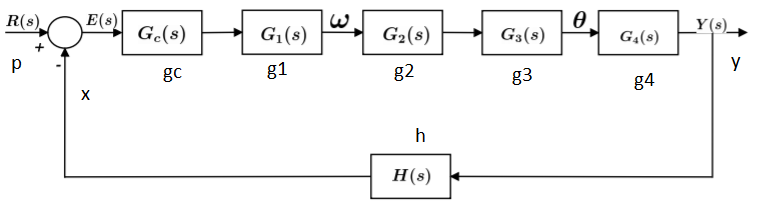
\includegraphics[width=125mm]{DiagramaBloques2.png}}}
            \caption{Diagrama de bloques para función en Maxima}
            \label{DiagramaBloques2}
\end{figure} 

En Maxima se logró comparar el resultado de la función de transferencia que se obtuvo en la sección anterior con el código mostrado en la figura \ref{max1}, y para lograr utilizar este código se tenia que tener en cuenta el diagrama de bloques mostrado en la figura \ref{DiagramaBloques2}, donde se puede apreciar que p es la entrada, y la salida, y x es la señal que viene de la realimentación. Donde $x=h.y$ y $y$ es la multiplicación de todos los bloques junto con $(p-x)$.

\begin{figure}[H]
            \centering
            \centerline{\centerline{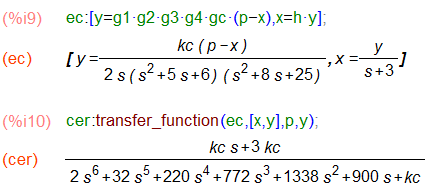
\includegraphics[width=125mm]{max1.png}}}
            \caption{Código de función de transferencia}
            \label{max1}
\end{figure} 

Para el error de estado estacionario se utilizó la función presente en la \ref{errorES}.

\begin{figure}[H]
            \centering
            \centerline{\centerline{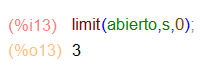
\includegraphics[width=125mm]{errorES.png}}}
            \caption{Código de error de estado estacionario}
            \label{errorES}
\end{figure}

Para el criterio de estabilización de Routh-Hurwitz se utilizó el código presente en la \ref{RHz}. Se puede observar como se van realizando las determinadas iteraciones para el calculo de la K y volver dar como resultado un rango de K con una mayor estabilidad, donde en ese rango se encuentra el valor correcto que se obtiene con un sobreimpulso menor al 5\%.

\begin{figure}[H]
            \centering
            \centerline{\centerline{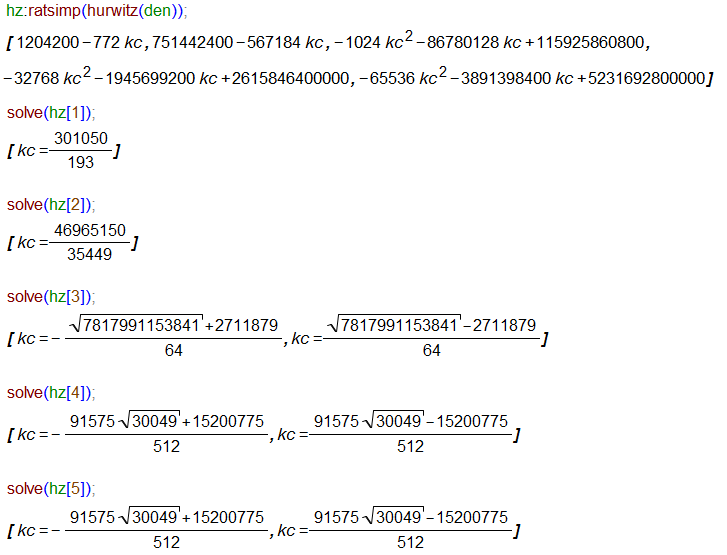
\includegraphics[width=150mm]{RHz.png}}}
            \caption{Código para criterio de estabilización de Routh-Hurwitz}
            \label{RHz}
\end{figure}

  \begin{figure}[H]
            
            \centerline{\centerline{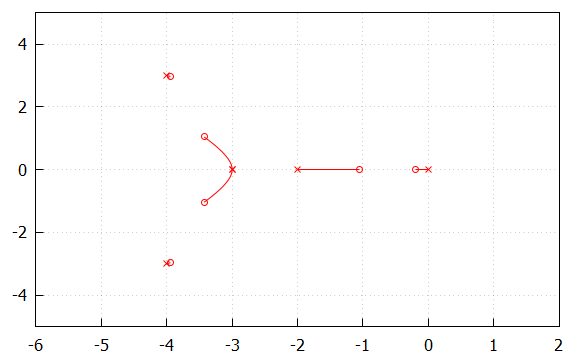
\includegraphics[width=125mm]{RL.png}}}
            \caption{Lugar de las Raíces}
            \label{RL}
\end{figure} 

En el lugar de las raíces visto en la \ref{RL}, se puede ver como existen 6 ceros y 5 polos, sin embargo para llevar a cabo la cuenta de los impares y los pares se termina dedcuciendo que en el polo -3 deben existir dos. El código utilizado para esto se presenta en la \ref{RLcode}.

\begin{figure}[H]
            \centering
            \centerline{\centerline{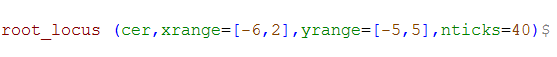
\includegraphics[width=125mm]{RLcode.png}}}
            \caption{Código para obtención del lugar de las raíces}
      \label{RLcode}
\end{figure} 


 \begin{figure}[H]
            \centering
            \centerline{\centerline{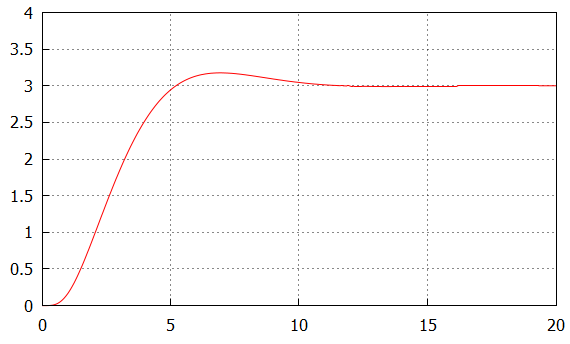
\includegraphics[width=125mm]{kc.png}}}
            \caption{Gráfica de Kc}
            \label{kc}
\end{figure} 

 \begin{figure}[H]
            \centering
            \centerline{\centerline{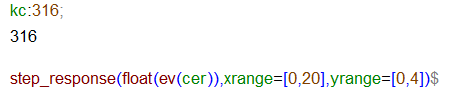
\includegraphics[width=125mm]{graficakc.png}}}
            \caption{Código para graficar la respuesta al escalón}
            \label{codgraf}
\end{figure} 

Podemos observar en la \ref{kc} como el Kc con un valor de 316 obtiene un resultado que se ve reflejado en el gráfico de la figura anterior, donde posee un sobreimpulso menor al 5\% y luego desciende. La \ref{codgraf} presenta el código utilizado para obtener esta gráfica de respuesta al escalón.

 \begin{figure}[H]
            \centering
            \centerline{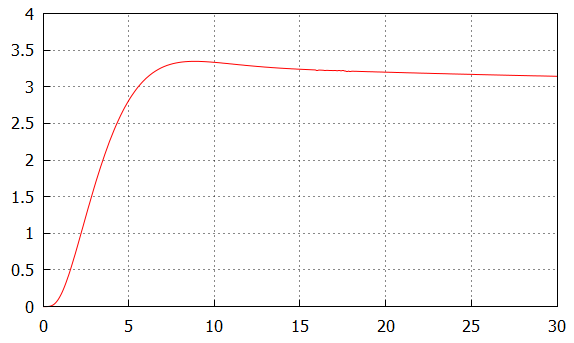
\includegraphics[width=125mm]{kcat.png}}
            \caption{Gráfica del compensador de atraso}
            \label{gca}
\end{figure} 

Según la imagen de la \ref{gca}, podemos apreciar como el compensador de atraso está realizando su trabajo para ralentizar el proceso de caída de la pendiente hasta llegar a la estabilización. 


 \begin{figure}[H]
            \centering
            \centerline{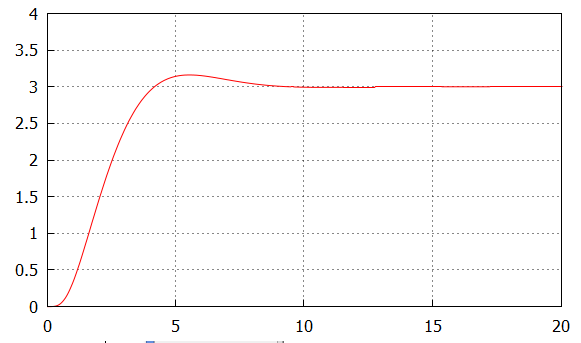
\includegraphics[width=125mm]{kad.png}}
            \caption{Gráfica del compensador de adelanto}
            \label{kad}
\end{figure}

En la \ref{kad} se puede observar como la posición en el tiempo de llegar a un máximo sucede en un tiempo mucho menor al escalón expuesto para el K de 316, donde claramente se puede visualizar en donde al momento 5 en la \ref{kc} aún no llega a su máximo y en la \ref{kad} ya tiene dicho valor en máximo, de esta manera explicando el comportamiento que le brinda un compensador de adelanto al sistema. Además de alncanzar dicho valor de sobreimpulso antes, se estabiliza en un tiempo menor al sistema sin compensador.

 \begin{figure}[H]
            \centering
            \centerline{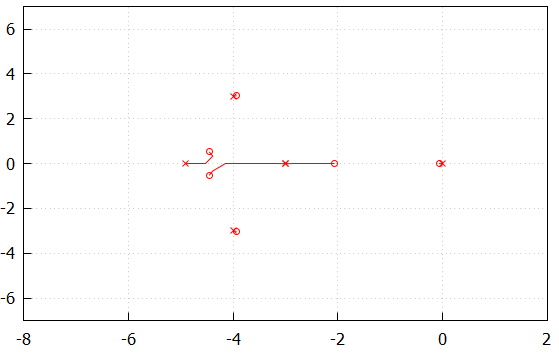
\includegraphics[width=125mm]{RLadel.png}}
            \caption{Lugar de las raíces con compensador de adelanto}
            \label{RLadel}
\end{figure}

En la \ref{RLadel} podemos observar como queda el lugar de las raíces con el compensador de adelanto. De manera que es visible que el polo que se unía a los ceros formando una media elipse, desaparece para colocarse por detrás. Además los polos y ceros conjugados que se encuentran detrás se colocan delante incluso de los ceros que se unían al polo en dicha forma.

 \begin{figure}[H]
            \centering
            \centerline{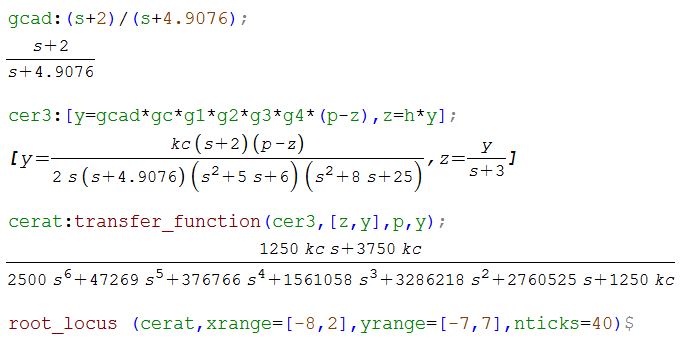
\includegraphics[width=130mm]{RLadelcode.png}}
            \caption{Código lugar de las raíces con compensador de adelanto}
            \label{RLadelcode}
\end{figure}

 \begin{figure}[H]
            \centering
            \centerline{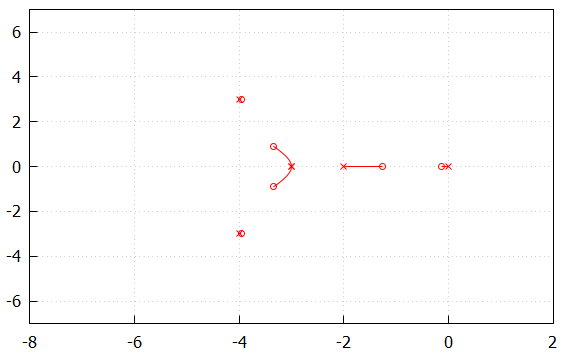
\includegraphics[width=125mm]{RLadel2.png}}
            \caption{Lugar de las raíces con compensador de adelanto con ts menor a 0.1}
            \label{RLadel2}
\end{figure}

Con la \ref{RLadel2} queda claro como se puede observar el lugar de las raíces con un compensador de adelanto en un tiempo de estabilización de 0.1s. Es evidente el cambio con la \ref{RLadel}, ya que el tiempo de estabilización empleado para dicho compensador es de 1.43s. De esta manera cambiando de manera drástica el lugar de las raíces y obteniendo un resultado distinto.

 \begin{figure}[H]
            \centering
            \centerline{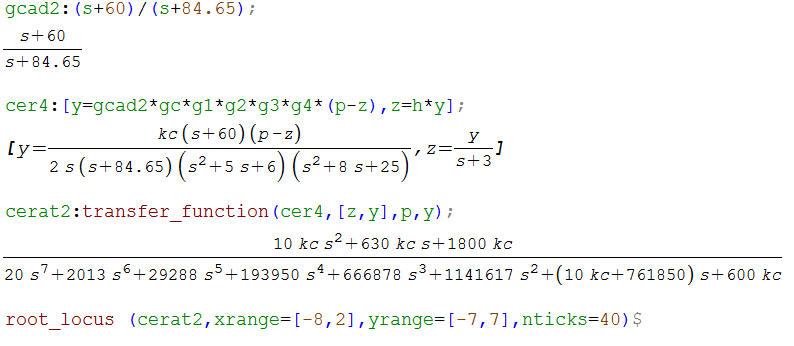
\includegraphics[width=150mm]{RLadelcode2.png}}
            \caption{Código lugar de las raíces con compensador de adelanto con ts menor a 0.1}
            \label{RLadelcode2}
\end{figure}

\begin{figure}[H]
            \centering
            \centerline{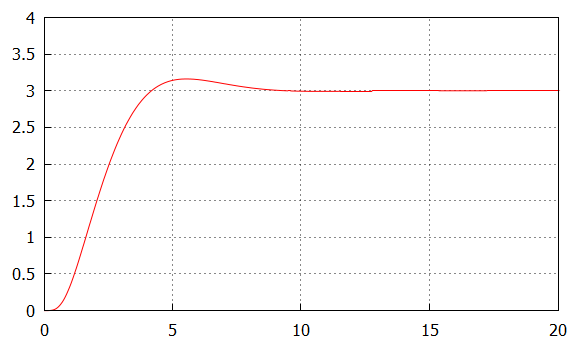
\includegraphics[width=125mm]{RLadel3.png}}
            \caption{Escalón obtenido con compensador de adelanto con ts menor a 0.1}
            \label{RLadel3}
\end{figure}

\begin{figure}[H]
            \centering
            \centerline{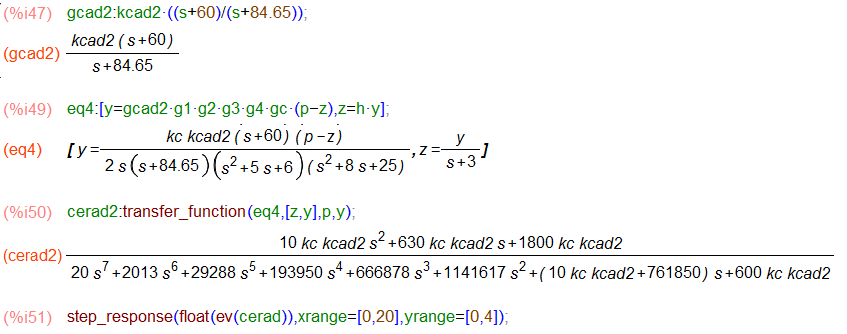
\includegraphics[width=150mm]{RLadelcode3.png}}
            \caption{Código del escalón obtenido con compensador de adelanto con ts menor a 0.1}
            \label{RLadelcode3}
\end{figure}

\section{Conclusiones}
\begin{itemize}
    \item El compensador de adelanto hace que el sistema llegue al punto máximo más rápido y que además logre una estabilización más pronta mientras que el compensador de atraso hace lo contrario. 
    \item El lugar de las raíces no se logró obtener como se habia planteado al hacer el procedimiento que se aprendio en clase, e incluso es pueden observar que existe un grave error ya que aparecen 5 ceros cuando solo existe 1 en el sistema. Esto puede ser posiblemente porque el software es un código libre y pueden haber problemas en el código creado por terceros.
    \item El compensador de adelanto obtenido mediante un tiempo de estabilización de 0.1s logra mantener una forma similar al lugar de las raíces que se obtiene con la respuesta al escalón obtenido con la constante Kc, mientras que el compensador de adelanto con un tiempo de estabilización de 1.43s, da como resultado un lugar de las raíces sumamente distinto, debido a los tiempos de estabilización. 
    \item Observando los tiempos de las diferentes respuestas al escalón obtenidas de las diferentes funciones de transferencia, para el mayor entendimiento de los tiempos, es notorio que se encuentra en la unidad de decisegundos, esto calculado con las diferentes reacciones de acuerdo a los compensadores que tenga conectado en serie el sistema.
    \item Es importante tener siempre en cuenta la teoría en cualquier proceso de diseño, ya que eso permite detectar posibles soluciones no eficientes o que sean incorrectas, a tiempo, y así, optimizar el tiempo lo más posible, ya que eso es un recurso muy valioso en ingeniería.
    \item La selección del polo o del cero en el compensador ya sea de adelanto o de atraso que se quiera diseñar, si se realiza estratégicamente, puede llegar a reducir los cálculos y el error humano a equivocarse dentro de los mismos, de manera considerable.
    
\end{itemize}

\section{Referencias} \\
[1] K. Ogata. Ingeniería de control moderna. 5ta edición. Madrid: PEARSON EDUCATION, S.A., 2010.\\
\\
[2] R.C. Dorf, R.H. Bishop. SISTEMAS DE CONTROL MODERNO. 10ma edición. Madrid: PEARSON EDUCATION, S.A., 2005.\\
\\
[3] Kuo, Benjamin C. Sistemas de Control Automático, Ed. 7, Prentice Hall,
1996, México.




\end{document}